%===================================================================================
% Chapter: Conclusiones
%===================================================================================
\chapter*{Anexo}\label{chapter:Anexo}
\addcontentsline{toc}{chapter}{Anexo}

  
%===================================================================================
\begin{figure}[h!]
	\centering
	\begin{subfigure}[b]{0.49\linewidth}
		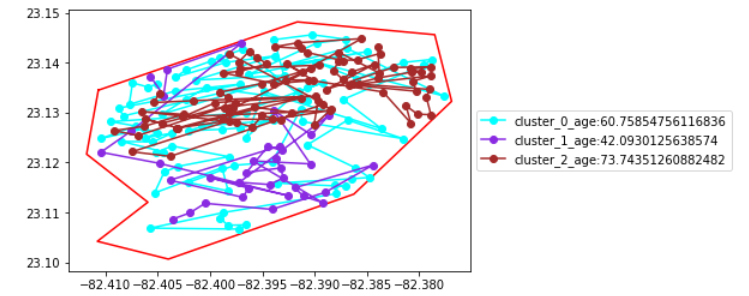
\includegraphics[width=\linewidth, height=3cm]{Images/Plaza.png}
		\caption{Plaza}
		\label{fig:Plaza}
	\end{subfigure}
	\begin{subfigure}[b]{0.49\linewidth}
		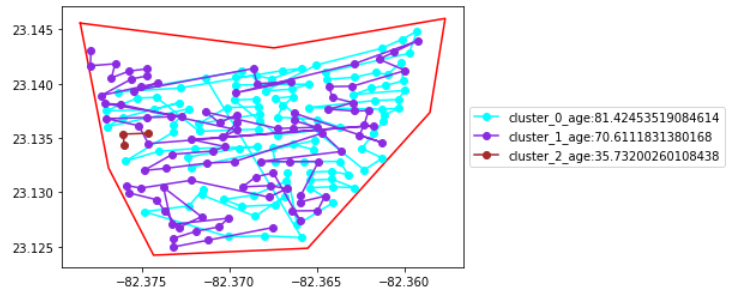
\includegraphics[width=\linewidth, height=3cm]{Images/CentroHabana.png}
		\caption{Centro Habana}
		\label{fig:CentroHab}
	\end{subfigure}
	\begin{subfigure}[b]{0.49\linewidth}
		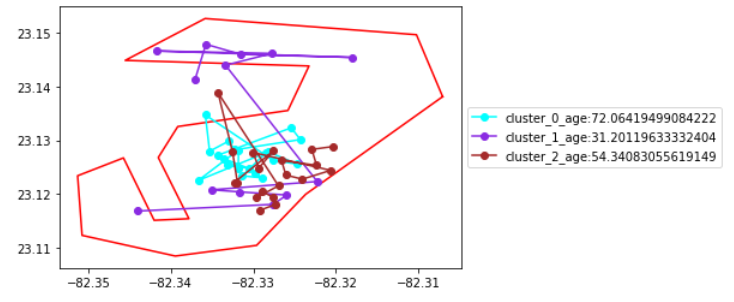
\includegraphics[width=\linewidth, height=3cm]{Images/Regla.png}
		\caption{Regla}
		\label{fig:Regla}
	\end{subfigure}
	\begin{subfigure}[b]{0.49\linewidth}
		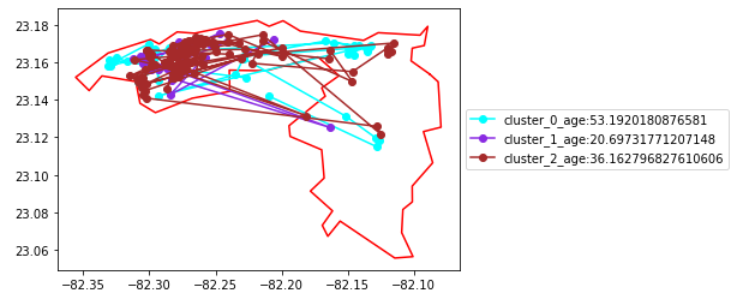
\includegraphics[width=\linewidth, height=3cm]{Images/HabEste.png}
		\caption{Habana del Este}
		\label{fig:HabEste}
	\end{subfigure}
	\begin{subfigure}[b]{0.49\linewidth}
		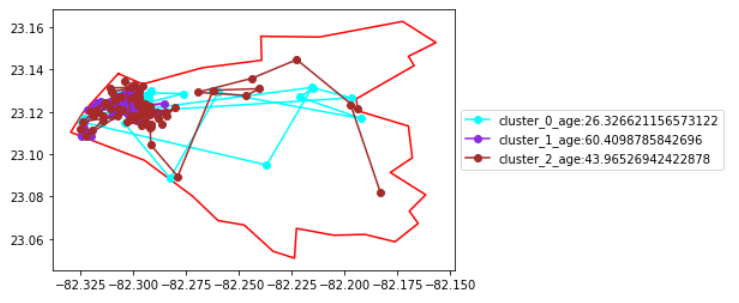
\includegraphics[width=\linewidth, height=3cm]{Images/Guanabacoa.png}
		\caption{Guanabacoa}
		\label{fig:Guanabacoa}
	\end{subfigure}
	\begin{subfigure}[b]{0.49\linewidth}
		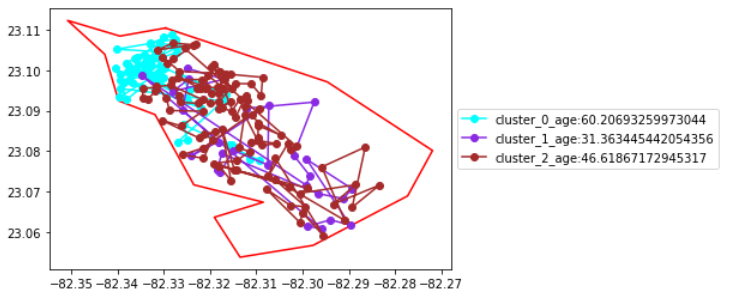
\includegraphics[width=\linewidth, height=3cm]{Images/SanMiguel.png}
		\caption{San Miguel del Padrón}
		\label{fig:SanMiguel}
	\end{subfigure}
	
	
	
	%\caption{Recorrido por el mapa}
	\label{fig:Resto de los municipios}
\end{figure}
\begin{figure}[h!]
	\centering
	\begin{subfigure}[b]{0.49\linewidth}
		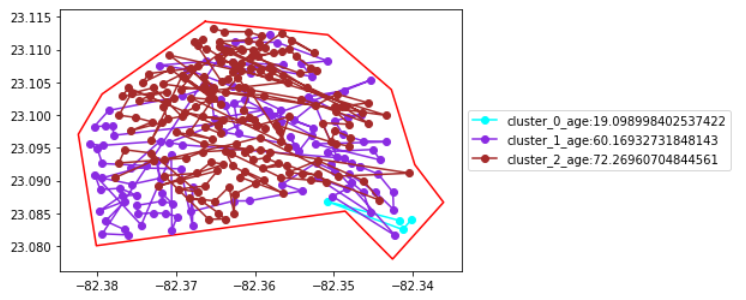
\includegraphics[width=\linewidth, height=3cm]{Images/10Otc.png}
		\caption{10 de Octubre}
		\label{fig:10Oct}
	\end{subfigure}
	\begin{subfigure}[b]{0.49\linewidth}
		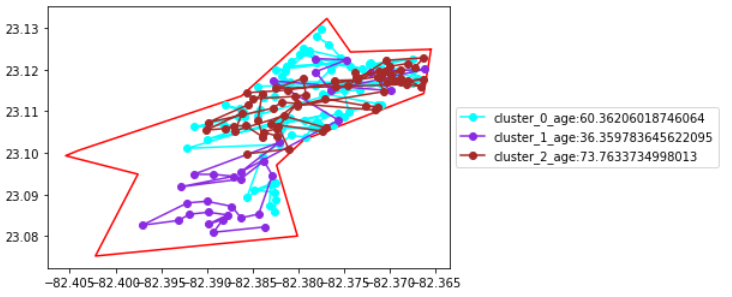
\includegraphics[width=\linewidth, height=3cm]{Images/Cerro.png}
		\caption{Cerro}
		\label{fig:Cerro}
	\end{subfigure}
	\begin{subfigure}[b]{0.49\linewidth}
		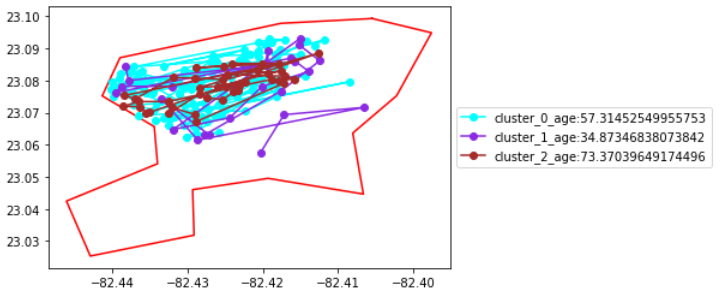
\includegraphics[width=\linewidth, height=3cm]{Images/Marianao.png}
		\caption{Marianao}
		\label{fig:Marianao}
	\end{subfigure}
	\begin{subfigure}[b]{0.49\linewidth}
		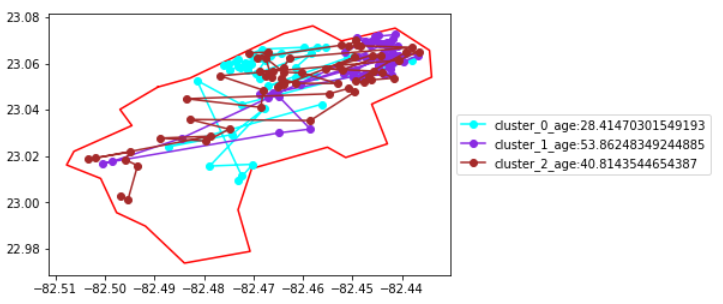
\includegraphics[width=\linewidth, height=3cm]{Images/LaLisa.png}
		\caption{La Lisa}
		\label{fig:Lisa}
	\end{subfigure}
	\begin{subfigure}[b]{0.49\linewidth}
		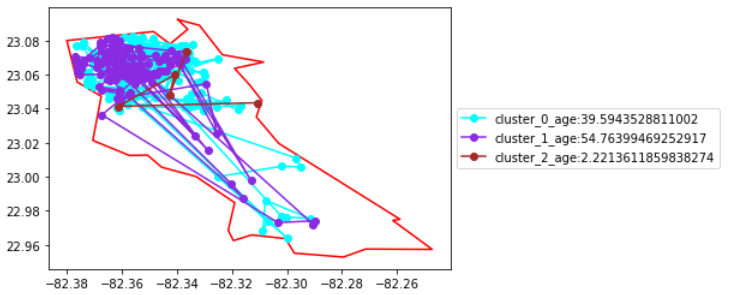
\includegraphics[width=\linewidth, height=3cm]{Images/ArroyoN.png}
		\caption{Arroyo Naranjo}
		\label{fig:Arroyo}
	\end{subfigure}
	\begin{subfigure}[b]{0.49\linewidth}
		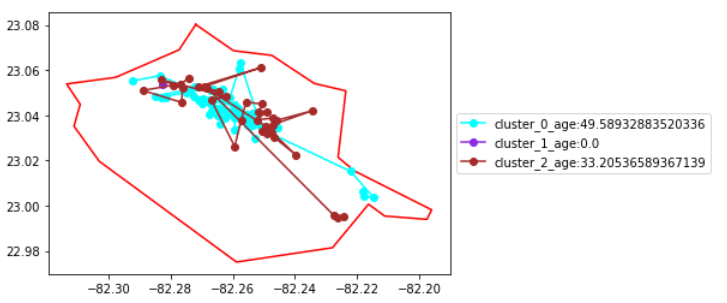
\includegraphics[width=\linewidth, height=3cm]{Images/Cotorro.png}
		\caption{Cotorro}
		\label{fig:Cotorro}
	\end{subfigure}
	
	%\caption{Recorrido por el mapa}
	\label{fig:RestoMunicipios1}
\end{figure}